\section {Evaluation}
Our model consists of three main components: CFG extractor for each app, 5UD-CFG embedding and the 3TU-CFG tensor embedding work based on the compressing and the clustering. We obtain the CFG extractor for each app, a open project Androguard \cite{Androguard}, which is disassembly tool to transform APK files to SMALI code. It is a disassembler for Android's DEX format. We implement 5UD-CFG embedding and 3TU-CFG tensor embedding work in numpy of Python, and achieve brute-force KNN searching in nearpy of Python. 


We evaluate our approach on five typical third-party Android markets: PP market, Xiaomi markets, Baidu markets , Tencent markets , Huawei markets.  We performed a effective analysis for the app homology. Our experiments are conducted on a server with 16 GB memory, 12 core at 1.6GHz and 7 TB hard drives.  All the evolutions are conducted based on five app datasets: 1) game app dataset; 2) social app dataset;  3) entertainment app dataset; 4) finance app dataset; 5) other app dataset. We let each type's app dataset as a kind of app community.

\subsection{Dataset}
\textbf{Dataset I - Game app dataset.} This data set mainly contains all kinds of game. Size of most games is more than $50 MB$, some even is more than $150 MB$. Game apps are nearly larger than other apps. We collect $32, 554$ apps from five Android markets, including $37\%$ hot game apps according to the rank and download rate. 

\textbf{Dataset II - Social app dataset.} This data set is the chat app, which has more links with others. This kind of app has more hidden threatens. Size of social app is from $20MB$ to $60MB$. The social app in other app types is the middle size. We collect $23, 295$ social apps from five Android markets.

\textbf{Dataset III - Entertainment app dataset.} Entertainment app dataset includes sing apps, photography apps, video apps, reading apps and etc. This kind of app enriches people's life, which is smaller than other app datasets. Size of entertainment app from $10MB$ to $50MB$. We collect $43, 885$ entertainment apps from five markets.

\textbf{Dataset IV - Finance app dataset.} Finance app dataset includes shopping apps, banking apps and etc. Many malware advertisements can be added in repacking finance apps. We collect $22, 846$ finance apps. %from five Android markets.

\textbf{Dataset V - Other app dataset.} Other app dataset includes utility apps, life apps and etc. Other apps mostly are from the unknown developer. This kind of app exists more serious threatens. We collect $30, 209$ other types' apps from five Android markets.

\subsection{App Homology Analysis Comparison}
We compare the 3TU-CFG tensor embedding work based on the 5UD-CFG embedding result with existing methods. All evaluations are conducted under the above five app datasets. We use the above five app datasets to train the homology dataset. We use the metric of the false positive rate to evaluate the accuracy. %We perform two time metrics to indicate the efficiency of the proposed and the other compared works. 
3TU-CFG Embedding time and the search time respectively represents the preparation efficiency and the search efficiency. 

%The number of apps in the same type group and the number of app class, which can also be called the app community, give a direct impression on the app detection in Android markets. The different community groups nearly does not share the same code. We also need to define a threshold for the app homology degree, impacts the classification results. We use the threshold $\delta =0.91 $ to perform the cross-market app homology analysis. When $\delta =0.91$, the measured false positive rate through 120 manual examination of randomly selected the app community group is $ 1\%.$
We prepare three representative app clone analysis or bug search techniques to compare our evaluation: Binary search based the Centroid \cite{ChenLZ14}, Gemini based Neural Network \cite{LiuCZLXCS17}, Genius \cite{FengZXCTY16}. We will introduce these three approaches in appendix.

%We introduce the main idea for these three solutions as follows:
%\begin{enumerate}

%\textbf{Centroid \cite{ChenLZ14}:} The centroid-based approach shows the scalability and accuracy for the app clone. We implemented a centroid bug search method for the five markets. This paper used a geometry characteristic, centroid, of dependency graphs to measure the similarity between methods in two apps.
%
%\textbf{Gemini \cite{LiuCZLXCS17}:} Gemini shows a novel neural network-based approach to compute the embedding based on the control flow graph of each binary function. We set the same iteration number of neural network as $5$. According to the proposed method by this paper, we use the above five datasets to train the embedding database.
%
%\textbf{Genius \cite{FengZXCTY16}:} Genius is a bug search system based on the CFG, which can scalable search bugs in the cross-platform. Genius's source code is not available. We use the proposed method to generate $16$ codebooks, and then complete the search database. We compare accuracy and efficiency with our method.  
%\end{enumerate}
    
\subsection{Accuracy Comparison}
In this Section, we evaluate the accuracy of a two-hierarchies embedding model and search work. %We construct a testing dataset by randomly selecting a certain number of apps or collecting several novel samples. 
We train embedding feature database from all collective apps as the search database. According to five types' markets, we obtain five basic search databases. We randomly select one or several apps from the testing dataset as the input. We assume that it is unknown about testing apps' types. We respectively search the input as five basic search databases.  
%Based on the app decompilation and two hierarchies embedding process, we obtain 3TU-CFG embedding vector as the search databases according to Algorithm. 1 and Algorithm. 2. 
    
For the five search databases, we train $152, 789$ apps in total, which includes $7, 491, 123, 901$ methods.  Database I has the $1, 596, 096, 888$ methods. Database II has the $1,142,135,436$ methods. Database III has the $2, 151, 646, 861$ methods. Database IV has $1, 120, 121, 321$ methods. Database V has $1, 481, 123, 391$ methods.

For the testing dataset, we have two parts: a part of apps from the basic five databases, and another part is from the novel collective apps. The number of apps that are collected in the search database is $1495$. The number of novel collective apps is $587$. 

According to the proposed method, we can obtain one closest candidate for testing samples. It is not necessary to find a query for each search sample. Fig. 4 (a) shows the true positive rate (TPR) when we set different similarity thresholds in the method-level. If the similarity thresholds is less than $0.0057$, TPR in the method-level is more than $98.5\%$. If the similarity thresholds is less than $6.9\times 10^{(-5)}$, TPR in the method-level is more than $68.7\%$. The larger the similarity threshold is, the TPR is larger. When the distance is more than the similarity threshold, we judge those two methods are not same. According to the proposed method, we find that different apps are with a larger distance. Make sure the similarity apps have the smaller distance is more important. If the similarity threshold is set too  larger, some similarity apps may be defined as the different apps with a large probability. Therefore, TPR is decreasing with the similarity threshold decreasing. 

\begin{figure*}[hbt]
   \centering
   \subfigure[]{\label{1} 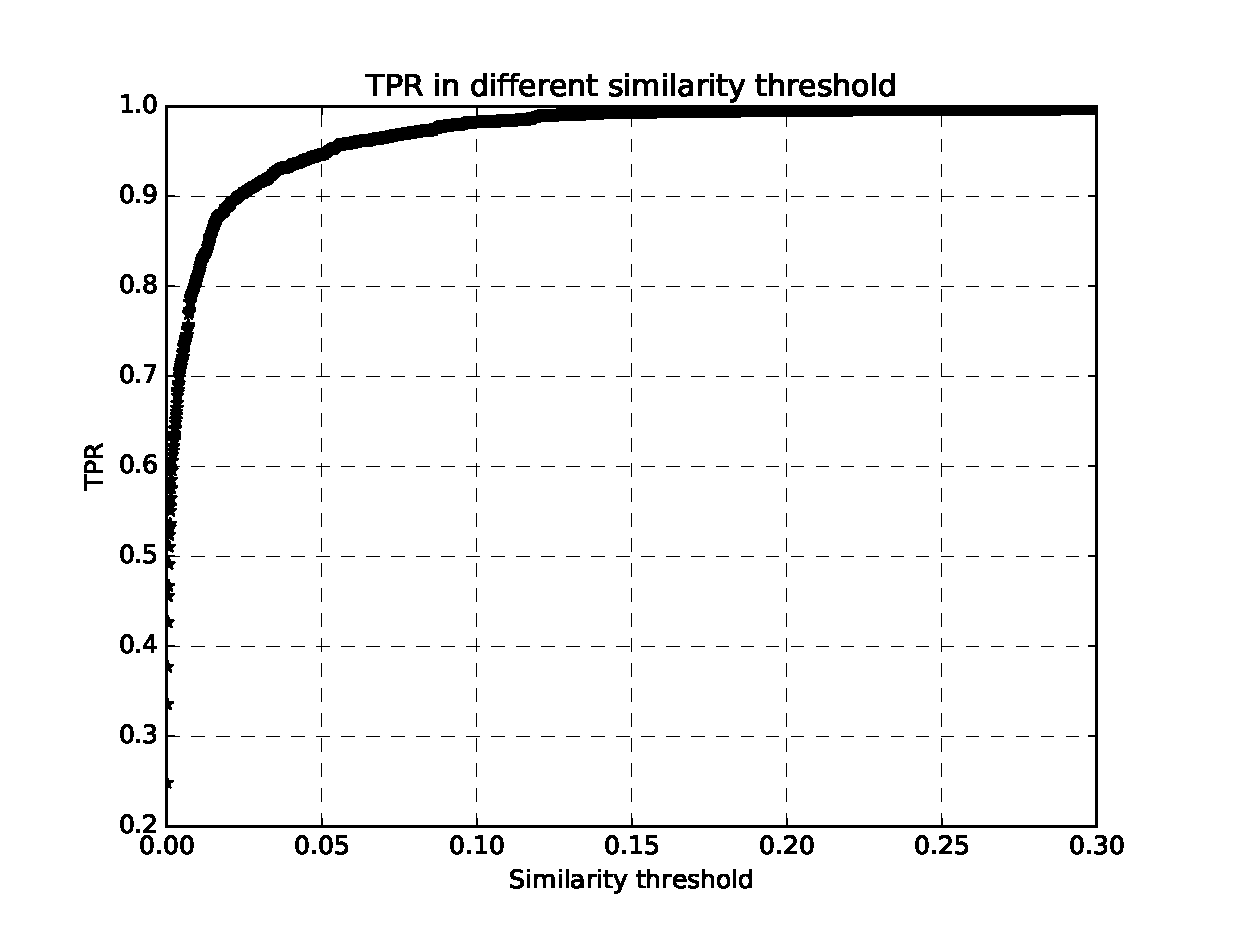
\includegraphics[width=0.30\textwidth]{threasholdcopy.eps}}
   \hspace{0.1in}
   \subfigure[]{\label{2} 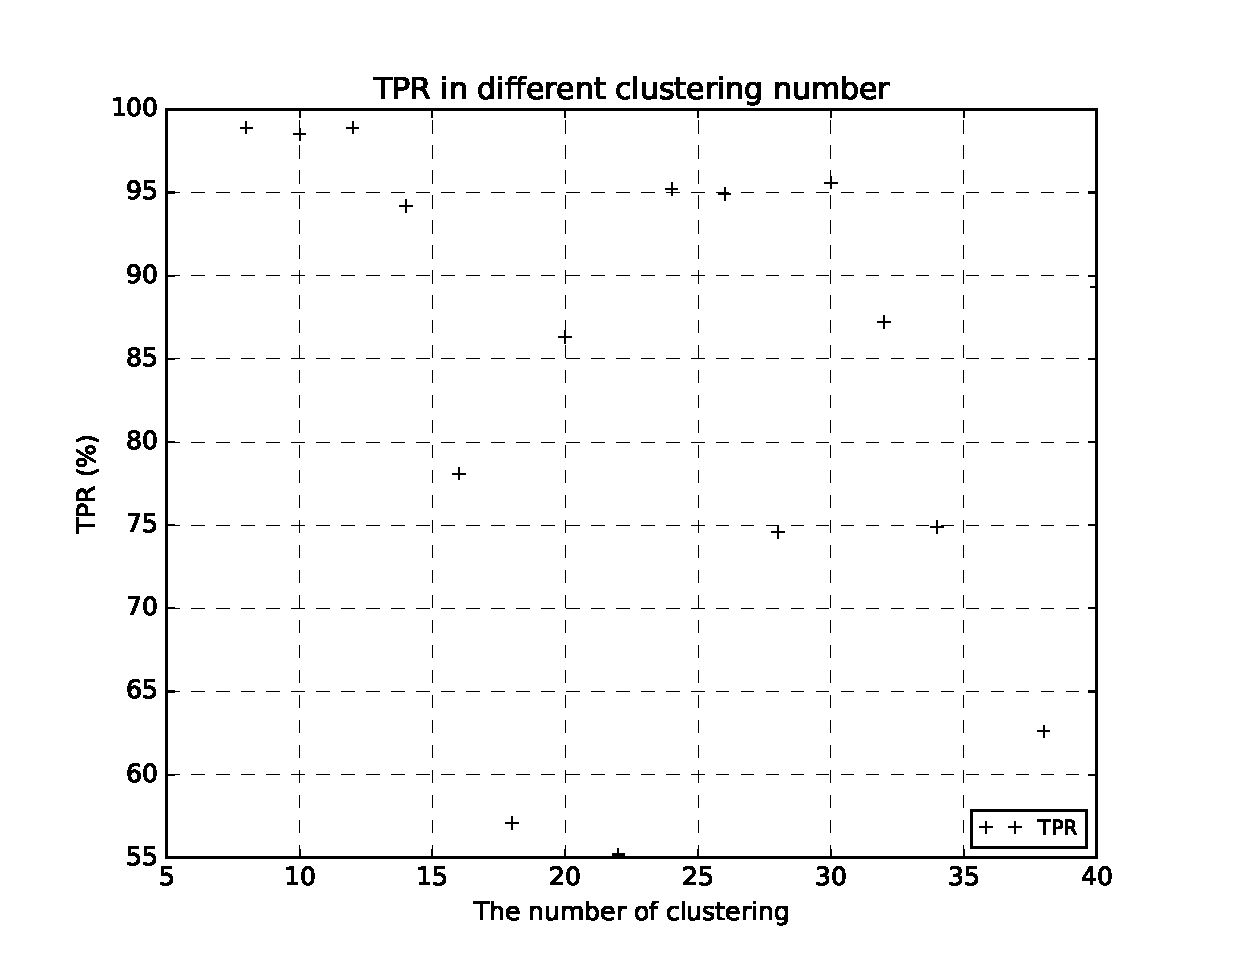
\includegraphics[width=0.30\textwidth]{clustercopy.eps}} \hspace{0.1in}
   \subfigure[]{\label{3} 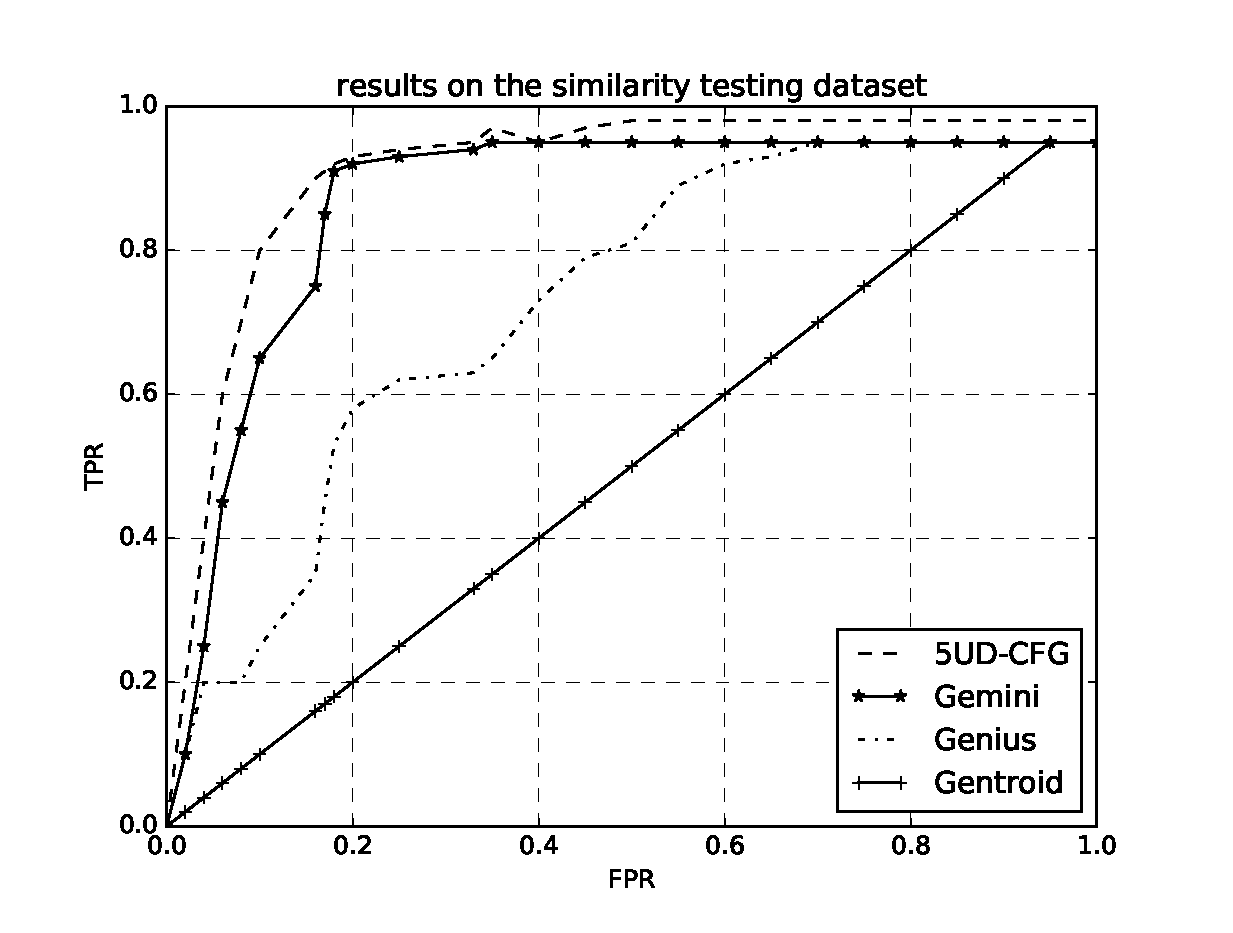
\includegraphics[width=0.30\textwidth]{TPRcopy.eps}}\\
   \caption{Accuracy}
   \vspace{-3 mm}
   \end{figure*}

%\begin{figure}[hbt]
%  \center{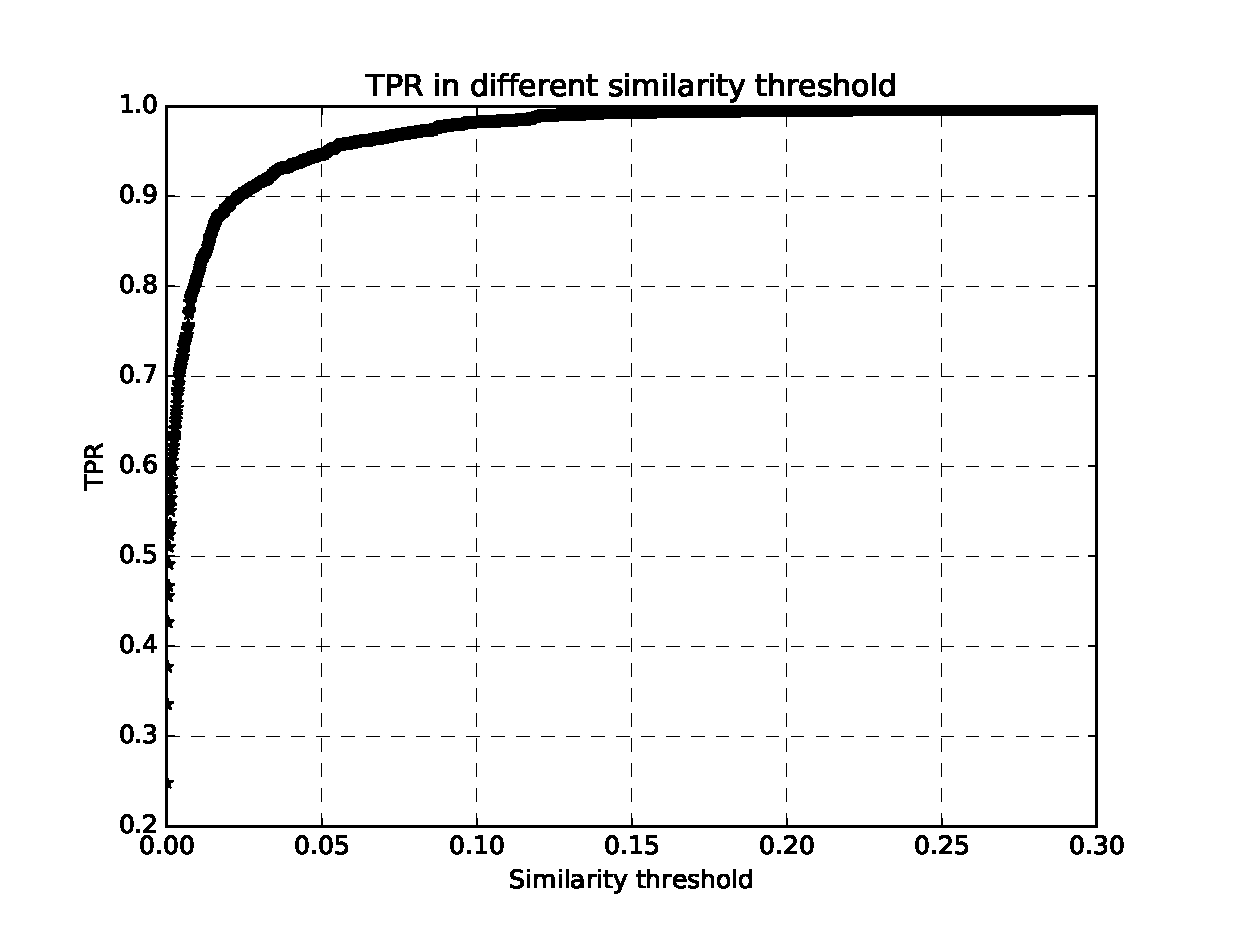
\includegraphics[width=8cm] {threasholdcopy.eps}}
%  \caption{\label{1}  TPR with different threashold}
%\end{figure}

Based on the proposed clustering algorithm in Algorithm 1, the different clustering's number affects TPR. Fig. 4 (b) shows that there is a inflection point in the changing curve of relationship between the clustering number and the TPR. We can see that TPR is the largest if the clustering number is $0.014\%$ of the number of search database. 
%\begin{figure}[hbt]
%  \center{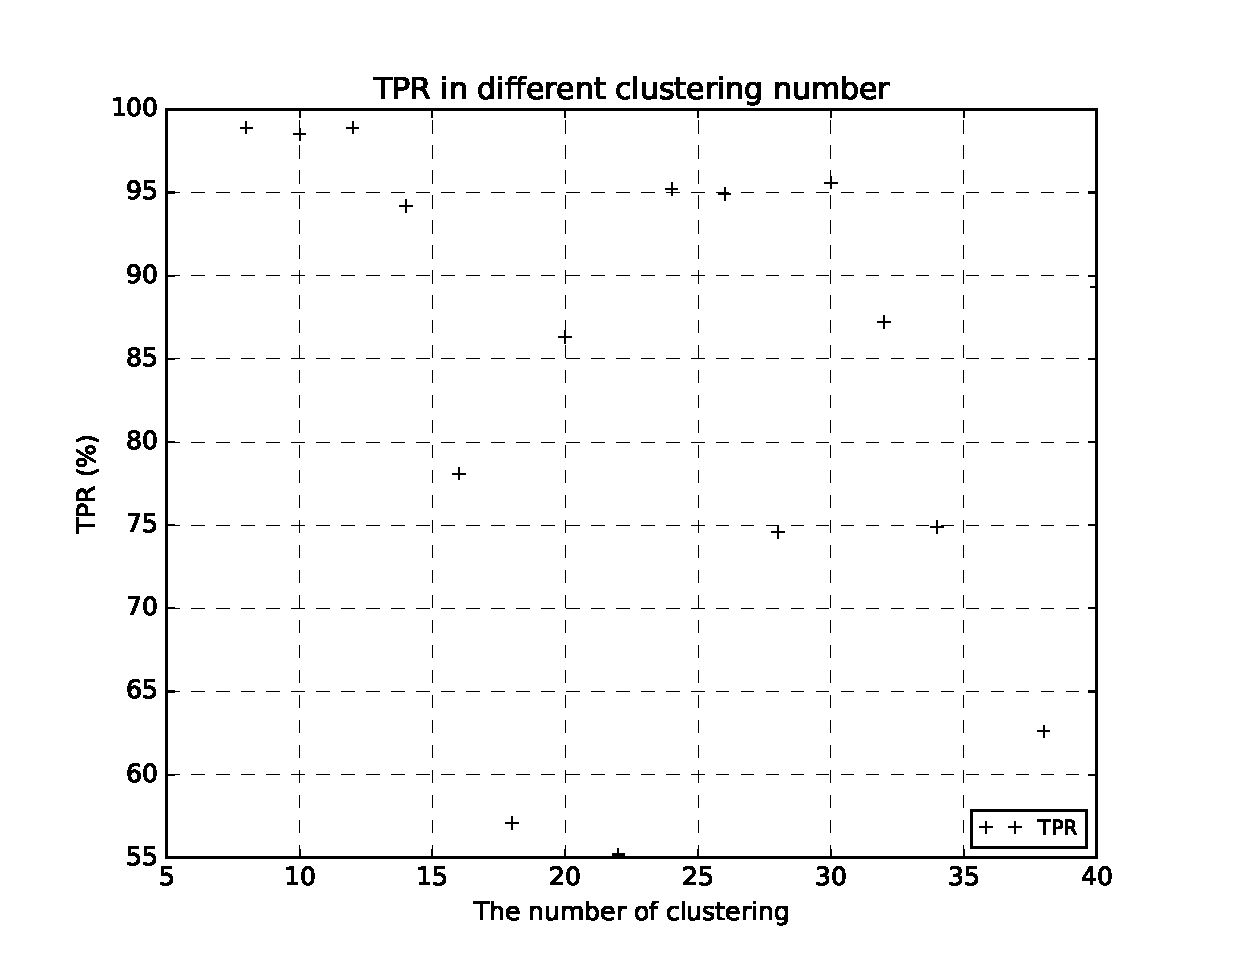
\includegraphics[width=8cm] {clustercopy.eps}}
%  \caption{\label{2}  TPR with different clustering number}
%\end{figure}

To compare the efficacy of final 3TU-CFG with centroid, gemini and genius, we use the same testing data to calculate the ROC curve in the same threshold. We use two metrics to evaluate the accuracy of the proposed and compared methods:the true positive rate (TPR) and the false positive rate (FPR). %For the searched samples query $q$, there are $m$ matching functions out of total of $L$ functions. If we set the first $F$ results as the positives, the total number of the correct matched functions $c$, which are true positive. The remaining number of functions in the $F$ functions, that is $F-c$, are false positives. We set the TPR as $TPR=\frac{c}{m}$ and the false positive rate is $FPR=\frac{F-c}{L-m}$. 

%\begin{figure}[hbt]
%  \center{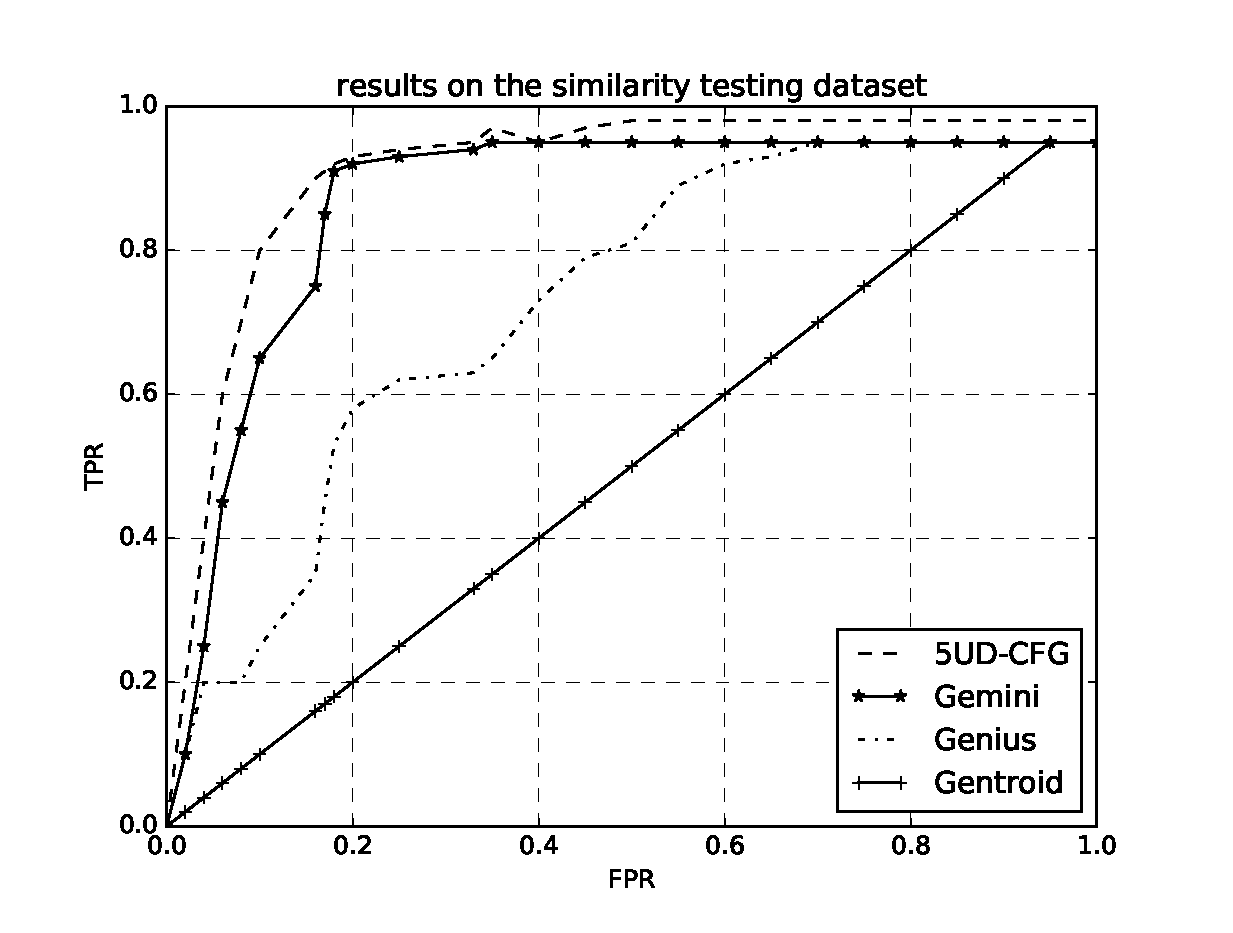
\includegraphics[width=8cm] {TPRcopy.eps}}
%  \caption{\label{3}  ROC on the similarity testing dataset}
%\end{figure}


%描述图7,比较三个方法。后面就是时间的实验部分。
We use $2082$ apps in the testing database as the queries to match with the target approaches. Fig. 4 (c) shows evaluating results of the ROC curve. we can see that 3TU-CFG outperforms another three approaches: Gemini, Genius, and Centroid. The size of ROC curve of 3TU-CFG is the largest, which shows the 3TU-CFG is the most accurate. When the FPR is small, TPR is significantly better than other approaches. Four curves show that TPR is increasing with FPR increasing. However, the rate of ROC curve of 3TU-CFG has the fastest growing. The results shows the 3TU-CFG can achieve even better accuracy than other approaches.

We consider search results and observe the advanced performance of 3TU-CFG is mainly because the 5UD-CFG can monotonously represent a function (proved in Section 4) and 3TU-CFG is obtained by monotonously compressing 5UD-CFG. Each function just need a closest candidate to make sure the accuracy for 3TU-CFG embedding process. The Gemini need train several iterations to get the embedding vector of the function. The model that is trained by the neural network needs a mount of samples to make sure the accuracy. Genius has several candidates that the accuracy depends on the accuracy of the codebook. Centroid has a great gap between different platforms, which is not monotonously represent the function. Our method is adept in representing entire structure of CFG, distinguishing the change, and thus shows the better results. 

According to our tensor model, we know that each benign function in a benign app have a benign label that denoted as $1$. If there is a malware function in a app, we consider this app is a suspicious app. For the suspicious apps found by our model, we validated them through online virus detection system and manual evaluations to judge the validity of our detection. 

%\subsubsection{Accuracy in the App Detection}
 
\subsection{Efficiency Comparison}
We measure the scalability of proposed approach from the following three aspects: the scale of the five collective markets, the performance on app homology detection and update of the basic feature database.

We analyze all apps in the collective five markets to obtain a basic database. Fig. 5 shows the distribution of size per app and the number for this app, the distribution of opcodes per app and the number for this kind of opcodes, and the distribution of the number of methods per app and the number for this app. We train in total $152, 789$ apps are in these five groups. Fig. 5 (a) shows that the size of nearly $94.7\%$  apps is in $0-50 MB$. The total size of apps is $7.47~TB$. The Fig. 5 (b) shows that nearly $69.8\%$ apps have $1-16000$ methods, and nearly $77.6\%$ apps have more than $4000$ methods.  

\begin{figure*}[hbt]
   \centering
   \subfigure[]{\label{1} 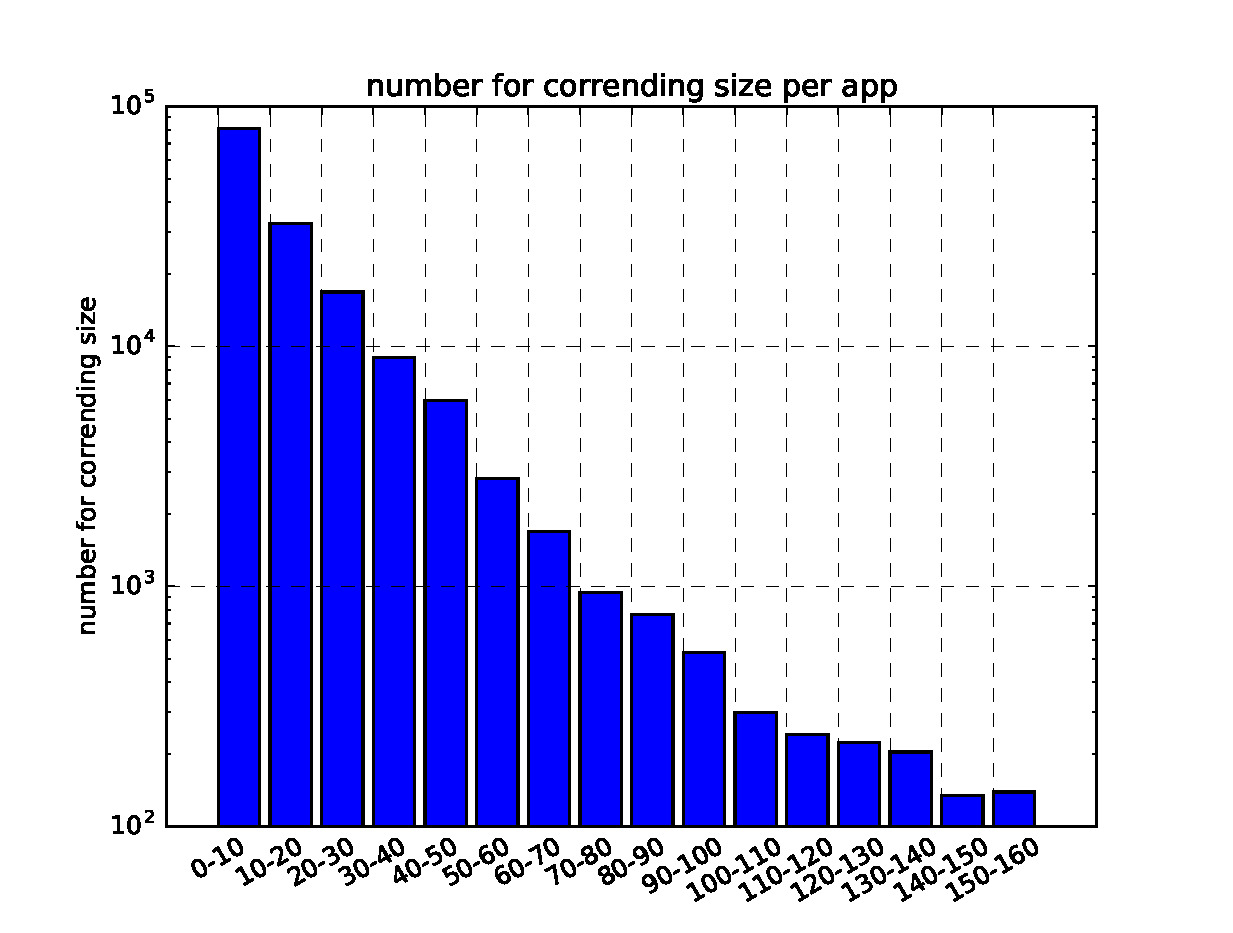
\includegraphics[width=0.30\textwidth]{numbercopy.eps}}
   \hspace{0.1in}
   \subfigure[]{\label{2} 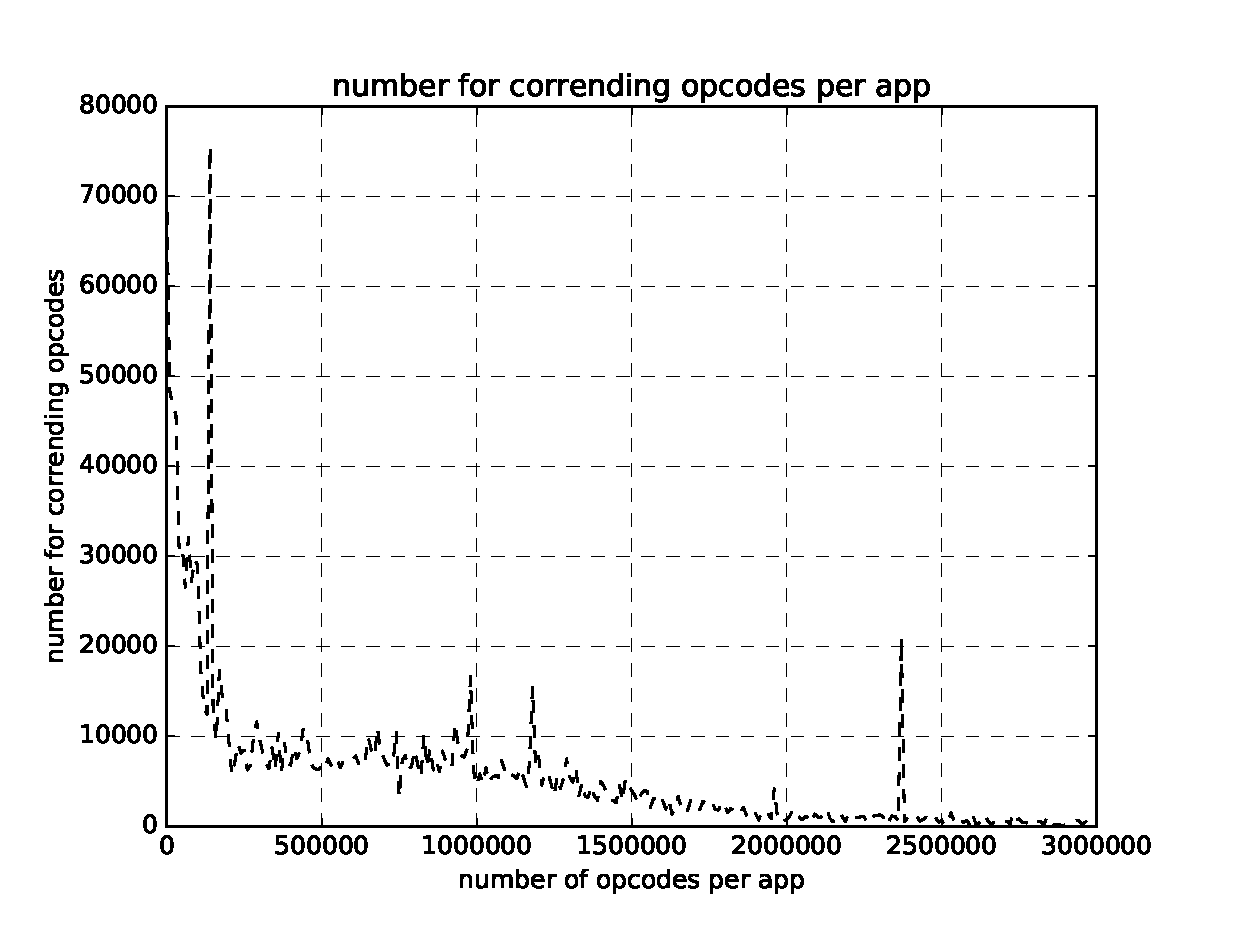
\includegraphics[width=0.30\textwidth]{opcodecopy.eps}} \hspace{0.1in}
   \subfigure[]{\label{3} 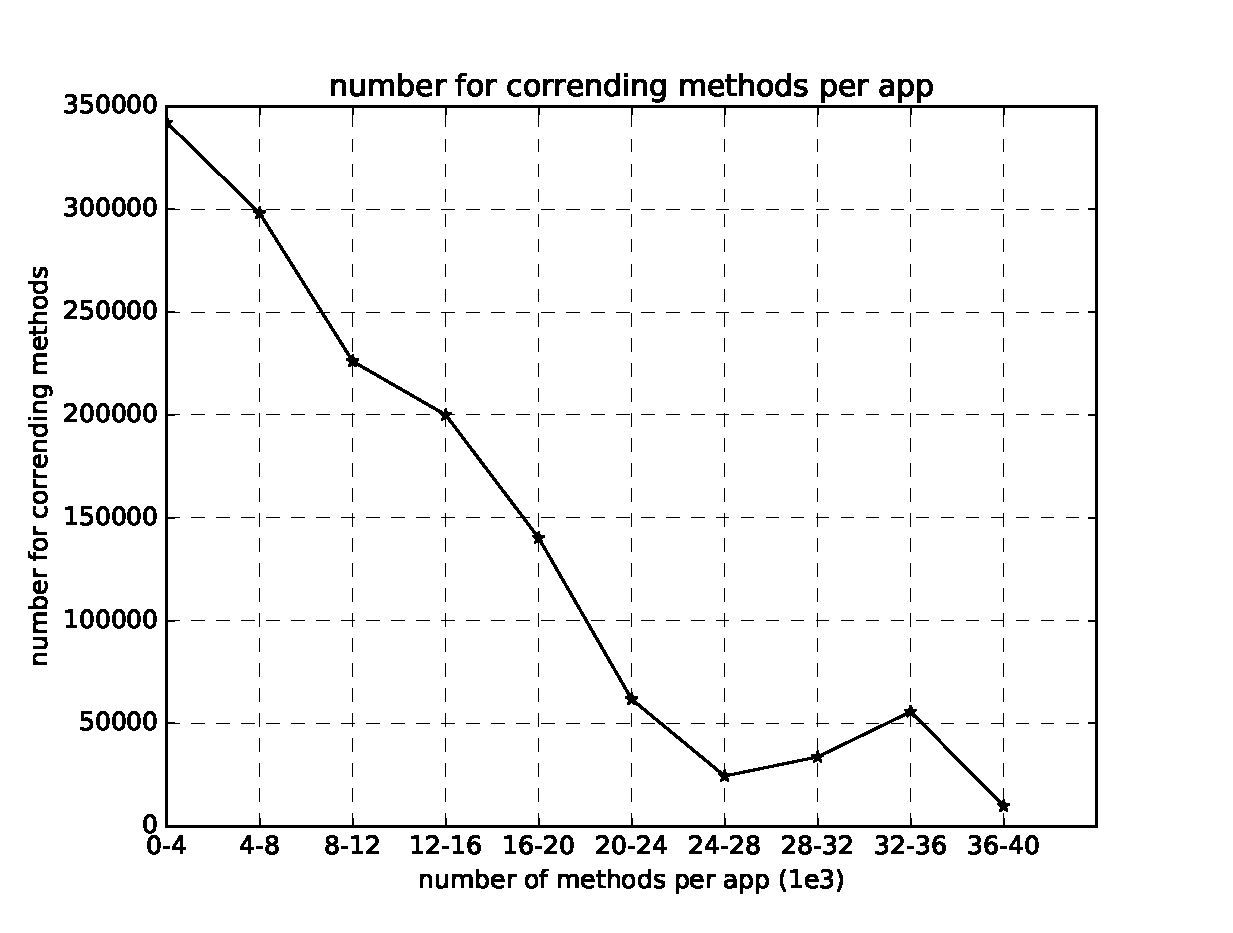
\includegraphics[width=0.30\textwidth]{methodcopy.eps}}\\
   \caption{Scalability of the database.}
   \vspace{-3 mm}
   \end{figure*}

We investigate the time consumption for each stage to demonstrate that 3TU-CFG is capable of handling apps at a large scale: 1) CFG with attributes extraction time, 2) embedding generation time, 3) Update time, and 4)app homology search time.

The time of the embedding generation depends on the total size of apps. We need to decompile the app into a series of functions. This step can be done in parallel. We use the androguard to obtain the original CFG structure. The original CFG generation time is the decompile time of the app. We can use several computer to measure the time. At the same time, Fig. 6 compare the 3TU-CFG embedding generation time with other three approaches, which including the decompile time. We store the CFG embedding vector in the database, and then use the KNN to search and detection. Then we evaluate the efficiency of Gemini, Genius for embedding time and Centroid for centroid generation time. 

\begin{figure*}[hbt]
   \centering
   \subfigure[]{\label{1} 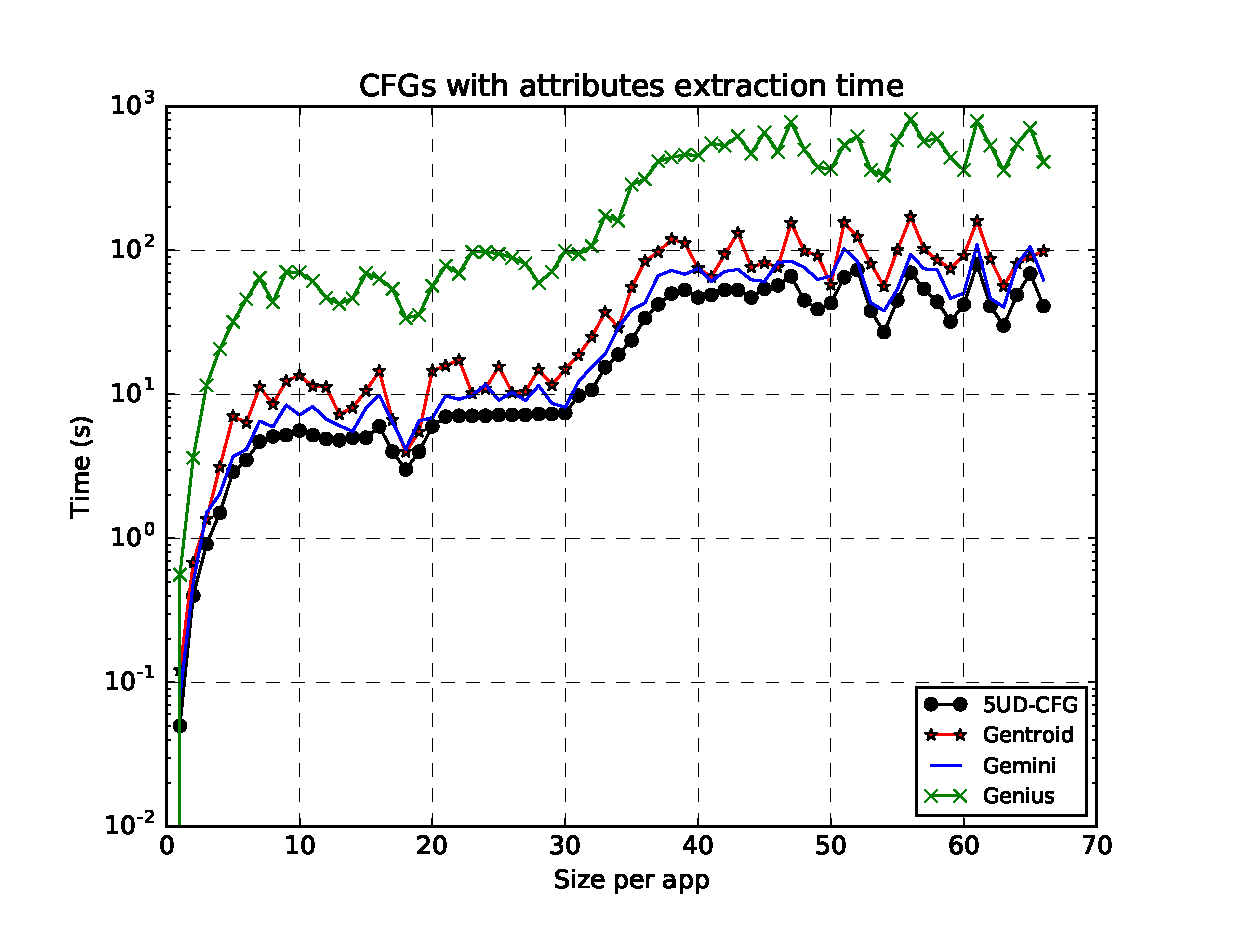
\includegraphics[width=0.30\textwidth]{extracttimecopy.eps}}
   \hspace{0.1in}
   \subfigure[]{\label{2} 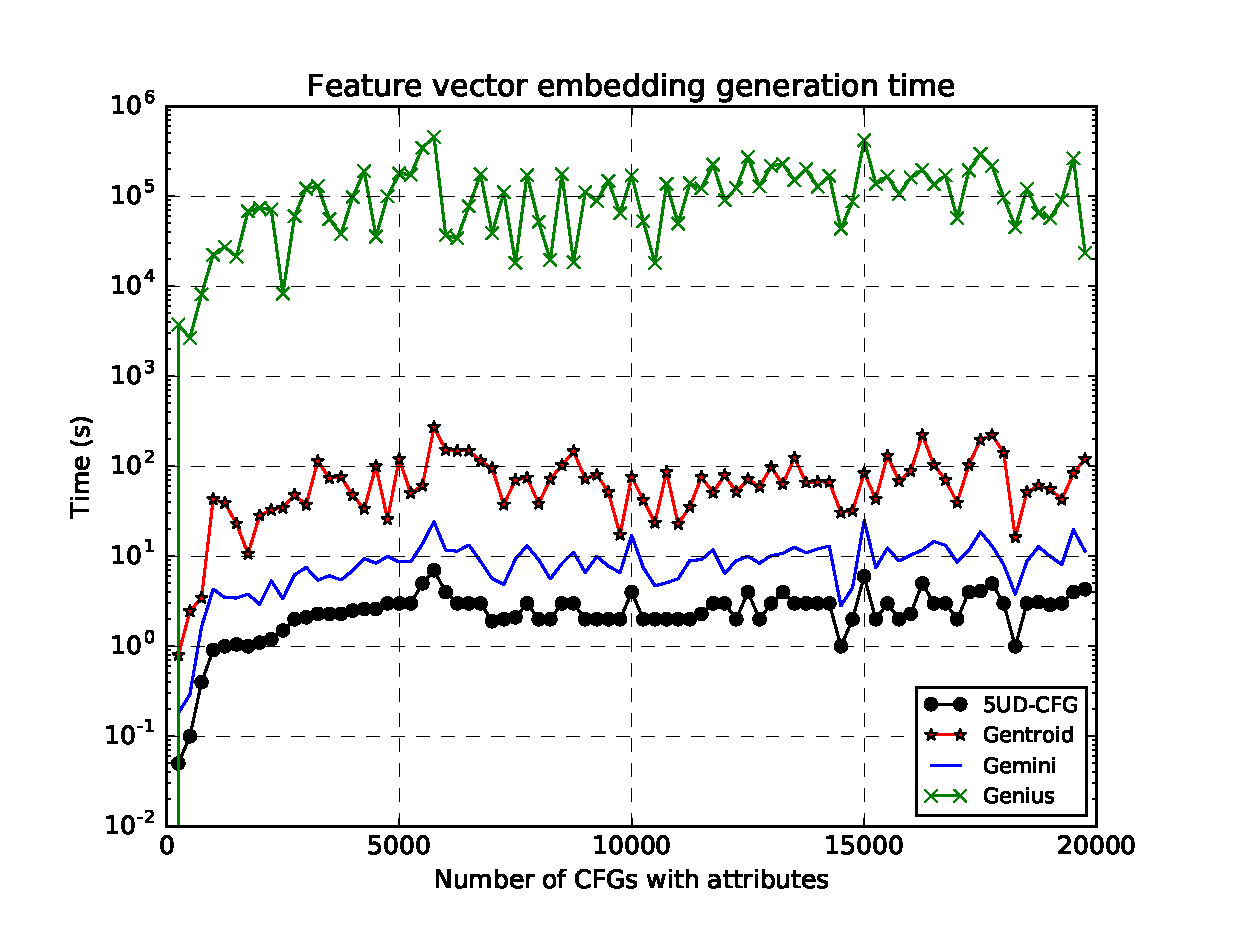
\includegraphics[width=0.30\textwidth]{embeddingtimecopy.eps}} \hspace{0.1in}
   \subfigure[]{\label{3} 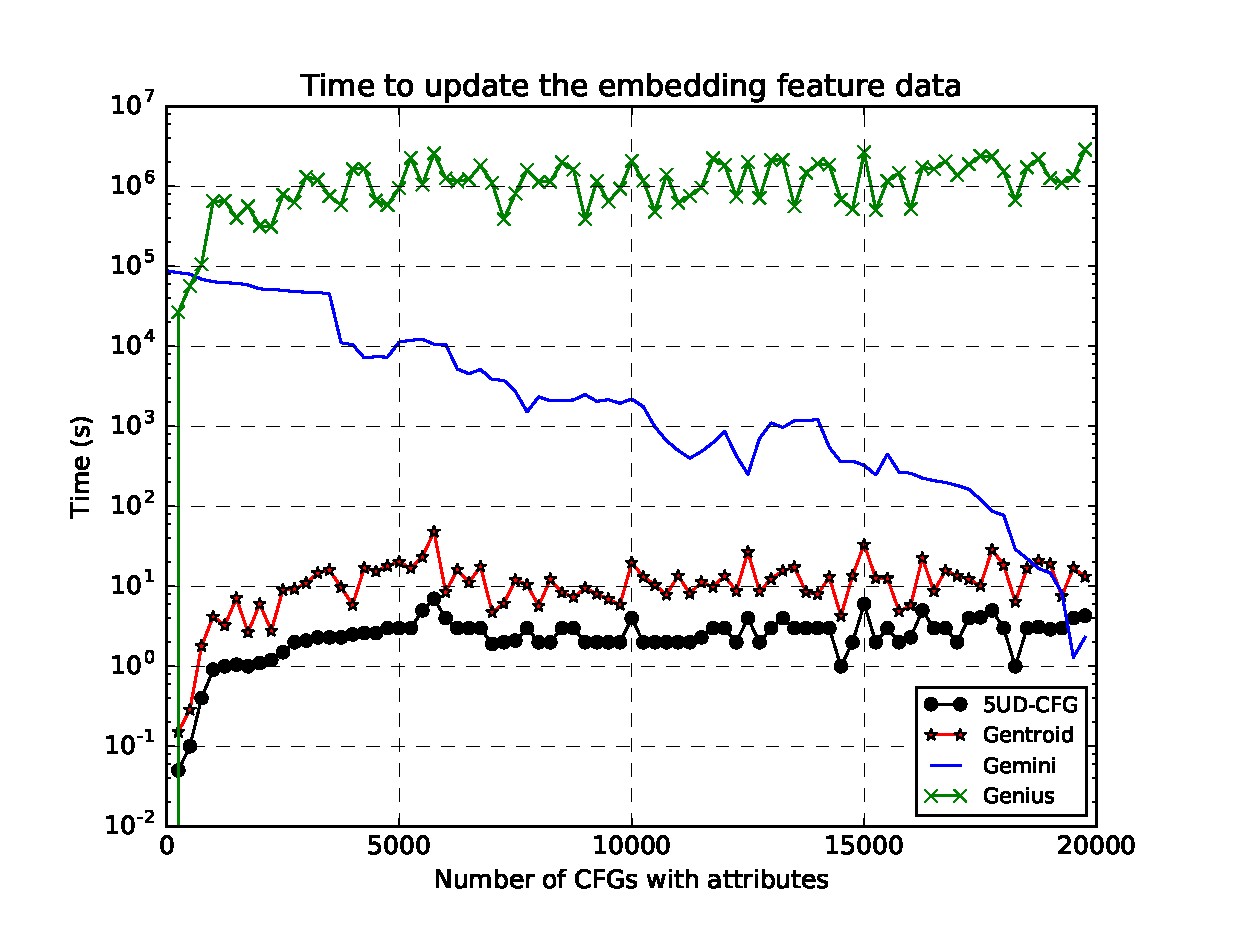
\includegraphics[width=0.30\textwidth]{updatetimecopy.eps}}\\
   \caption{Efficiency evaluation.}
   \vspace{-3 mm}
   \end{figure*}
 
 \begin{figure*}[!hbt]
   \centering
   \subfigure[]{\label{1} \includegraphics[width=0.30\textwidth]{searchtime_final.eps}}
   \hspace{0.1in}
   \subfigure[]{\label{2} \includegraphics[width=0.30\textwidth]{geniussearchtime_final.eps}} \hspace{0.1in}
   \subfigure[]{\label{3} \includegraphics[width=0.30\textwidth]{centroidseartime_final.eps}}\\
   \caption{Search time in scalable feature data.}
   \vspace{-3 mm}
   \end{figure*}


\subsubsection{Performance on CFG with attributes extraction time.}

Fig. 6 (a) shows the CFG with attributes extraction times of 5UD-CFG can improve upon Genius by $8\times$ to $15\times$ on average on CFG embedding time. The 5UD-CFG needs to extract 5 basic-block attributes along with the structure feature of the CFG. However, Genius needs to additionally extract the betweenness attributes, in total 8 attributes. The different becomes larger for the app with a large size. A app with the large size has more methods. There are more nodes in a CFG. It needs more time to compute the betweenness attributes for larger size's app with a amount of nodes. The preparation times of the 5UD-CFG can improve upon Gemini by $1.1\times$ to $1.7\times$ on average for different sizes of apps. Gemini needs to extract 6 basic-block attributes and the number of offspring time. However, Gemini aggregate the graph structural information through iterations of embedding update. Therefore, the CFG with attributes extraction times of the 3TU-CFG is close to Gemini. Centroid also extract 5 basic-block attributes with the structure feature, the process is similar to the CFG with attributes extraction process of the 5UD-CFG. The CFG with attributes extraction times of the 5UD-CFG is close to Centroid. 

\subsubsection{Performance on embedding generation time.}

Fig. 6 (b) shows the embedding generation time for four approaches with the increasing number of methods. The number of method denotes the scalable of the CFG. Obviously, more methods need more embedding time. 3TU-CFG, Genius, Gemini and Centroid all transform the CFG of the function to the embedding vector. We can see 3TU-CFG run $4700\times$ to $76000\times$ faster than Genius, run $2.1\times$ to $5\times$ faster than Gemini, and run $7\times$ to $51\times$ faster than Centroid on average. Since 3TU-CFG embedding process avoids the complexed neural network learning process, the expensive graph matching and the scalable clustering algorithm. Genius needs extra time to generate the codebook for all CFGs by the complex bipartite graph matching. Gemini needs extra time to learn five iterations for obtaining the CFG embedding feature. Centroid is to compute the centroid of a spatial geometry. This preparation process is simpler than the above two approaches. Therefore, the preparation time of Centroid is lower than another two approaches. However, the embedding process of the 3TU-CFG is more concise than other three approaches. The line embedding and the tensor embedding have much simpler matrix operations than that in the neural network iteration computation. However, Gemini and 3TU-CFG belong to the matrix operation, which can be parallelized.      


\subsubsection{Performance on Update time.}

Fig. 6 (c) shows the update feature database time. Adding new apps is very common in android markets. If the new app is not included in the database, we need to update the database. We can see that the update time of 3TU-CFG is quicker $4\times$ to $20000\times$ than Gemini, quicker more than $180000\times$ than Genius, and quicker $2\times$ to $7\times$ than Centroid. If we just update few apps at once, the different of time between the 3TU-CFG and the Gemini is larger. Since we propose a incremental algorithm of tenor embedding that just needs to retrain the increasing novel methods rather than retrain all feature vector. If the number of novel methods are same with the number of original feature data. The update embedding time of 3TU-CFG is close to Gemini. Since the Gemini need to embed all ACFGs to get the update feature data although it does not need to regenerate ACFGs. Specifically, Genius needs to retrain the codebook, this is a larger project, which means regenerate all feature vector including scalable graph matching algorithm. It costs too much time. Centroid just needs to update the increasing apps. However, it's accuracy is lower than the 3TU-CFG. Therefore, 3TU-CFG has a better performance on the update.
%We evaluate the scalability of 3TU-CFG on the collective five app markets, which consist of in total $152, 789$ apps. We investigate the time consumption for each stage to demonstrate that 3TU-CFG is capable of handling apps at a large scale. 

\subsubsection{App homology search time.} 
Fig. 7 (a) shows the search time for 3TU-CFG in the larger scale codebase. We choose five collective dataset into six codebases of different scales from $c=10^3$ to $c=10^8$, where $c$ is the total number of functions in the codebase. We choose the $1$ to $10000$ sequentially submitted queries. As we can see, the search time grows like linearly according to the increase of the codebase size, and the average search time is close to $4.6 \times 10^{(-9)}$. Fig. 7 (b) shows the search time for Gemini and Genius, these two approaches use the same propose LSH search method and the number of the feature vector are also same. Therefore, they have the same distribution of the search time. We can see the search time of the 3TU-CFG run $2\times$ faster than Genius and Gemini on average. Since the 3TU-CFG finally has a 3-eigenvalues vector, half as many as the feature vector of Genius and Gemini. The search method use the KNN search algorithm. Fig. 7 (c) shows the search time for Centroid, 3TU-CFG run $10\times$ to $100\times$. Since Centroid use the binary search for a 5-eigenvalues vectors, which is slower than KNN with a 3-eigenvalues vector. Therefore, 3TU-CFG has the less search time for scalable database.




%There have been several existing works for the function clone and other works for app clone:   

